\section{Preminaries\label{se:pre}}

This section first defines the concept of an application model to be mapped and scheduled. Further, the assumption of the target platform is presented. Finally, the problem to be optimized
is sketched.
\subsection{Weighted task graph}
In this paper, we concern coarse-grained application models. An application consists of a set of tasks with well-defined precedence constraints. Therefore, we adopt task graphs as the formulation~\cite{cotton2011multi}. To record the amount of work to be dealt with on a task, and data to be transferred, we assign weights on the tasks and data flows between different tasks, respectively.
\begin{defi}[Weighted Task Graph]
A weighted task graph is a tuple $G=\langle T,E\rangle$, where $T$ is a finite set of tasks, with $\delta: T\rightarrow \nn$ to indicate the amount of work to be dealt with on each task, and $E\subseteq T\times T$ is a set of precedence relations with $c: E\rightarrow \nn$ to indicate the amount of data transferred between each pair of tasks.
\end{defi} 

\begin{figure}
\centering
 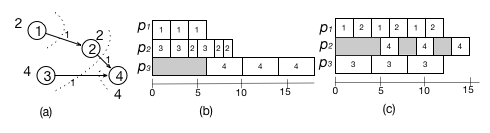
\includegraphics[width=0.85\columnwidth]{figures/taskgraph}
  \caption{A running example.}
 \label{fig:taskgraph}
 \vspace{-6.5mm}
 \end{figure}
 If there is no explicit precedence relation between a pair of tasks, the amount of communicated data is zero.  
 We also assume that the graph is acyclic. For an application with loops, we need to reduce it to acyclic graph by unfolding techniques. Take the model in Fig.~\ref{fig:taskgraph} as an example. There are four tasks, each of which is labelled with the amount of work, and three edges are labeled with the amount of transfered data. 

\subsection{Target platform}
We consider architectures connected with heterogeneous processors, each of which has a private memory, as shown in Fig.\ref{fig:platform}. Each processor can access its private memory directly, while accessing private memories of peer processors is not permitted. In order to communicate with peer processors, DMAs (Direct Memory Access) are implemented in the hardware platform. They can read from and write to all private memories under the control of processors. % each processor can access others through buses. %The DMA module takes charge of communication between the processors and off-memory. 
\begin{figure}
\centering
 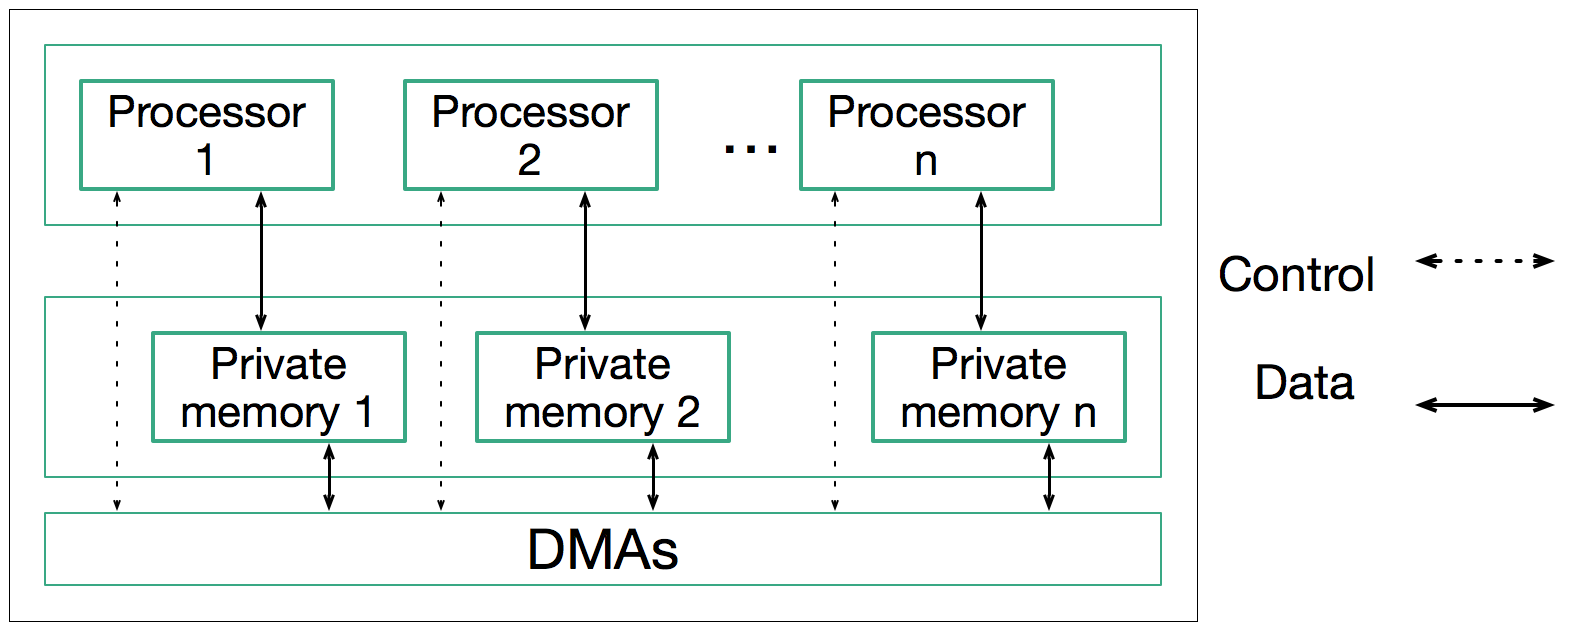
\includegraphics[width=0.8\columnwidth]{figures/platform.png}
  \caption{The target architecture.}
 \label{fig:platform}
 \vspace{-7.5mm}
 \end{figure}
We make the following assumptions for the target architecture:
\begin{enumerate}
%\item The architecture is fully connected.%, such that all the processors and the shared bus can be reached via any buses.
\item The cost for intra-processor communication is negligible. We only consider inter-processor communication.
\item A processor is occupied for initializing communication. Once the initialization is ready, the processor is released.
\item An inter-processor communication can start after the initialization. And multiple transmission to different destinations can be executed simultaneously. 
\item There is no memory access collisions.
\item Private memories are big enough for data storage.
\end{enumerate}

When the weight of a precedence relation in a task graph is greater than zero, and the two tasks are allocated to different processors, inter-processor communication is required. To simplify the model description, we restrict the communication architecture to a direct connection between different processors via inter-processor communication.

%To simplify the description of the constraints, we ignore the cost of task switch within the same processor.
\vspace{-8pt}
\subsection{Problem description}

%Given a task graph and a set of processors, 
We aim to construct static schedules for the target implementation. 
More precisely, the
tasks are statically allocated among the processors and
all executions (instances) of a task are executed on the same
processor, and no instance is permitted to migrate among
processors. Hence, mapping relations between tasks and processors are fixed during execution, and the sequences of task execution remain unchanged.

The tasks of an application will be repeatedly executed for a certain scenario.
%And the scheduling may be optimized after several iterations. 
Therefore, it is not enough to estimate the makespan of the whole with one time execution of the tasks. 
And we consider the minimisation of makespan within certain number of iterations. 


Given a task graph $G$ and a set of processors $P$, a mapping is a function $m: T \times P\rightarrow \bool$ with $m(t_i,p_k)=true$ meaning that task $t_i$ executes on processor $p_k$. 
Then the scheduling of tasks is a function $\tau: T\times \nn \rightarrow \nn$ with $\tau(t_i,u)=n$ meaning that the time of $u$th invocation of task $t_i$ is $n$. Suppose the function of processor speeds is $\rho: P\rightarrow \nn$. The duration of executing $t_i$ is $\kappa(t_i)=\delta(t_i)/(\sum^{|P|}_{k=1}\rho(k)*m(t_i,p_k))$. By abuse of notation, $\tau(t_i,u)$ is denoted by $\tau^u_i$ and others only use the subscripts instead. Then given the number of iterations $N$, the makespan is 
$${\cal{M}}=max \{i : \forall i ~\tau^N_i + \kappa_i\}.$$ 
The ideal situation for a balanced workload is that the workload on each processor is equal, i.e., 
%$\alpha=\dfrac{1}{|P|}*\sum^{|P|}_{k}  (\sum^{|T|}_{i} \delta_i *m_{i,k})/ \rho_k$. 
$aver= \sum^{|T|}_{i=1} \delta_i /|P|$. 
Hence, the difference between real workloads and the perfectly balanced workload is measure with $${\cal{W}}=\sum^{|P|}_{k=1} \mid\sum^{|T|}_{i=1}\delta_i*m_{i,k}- aver\mid.$$

Consider the example in Fig.~\ref{fig:taskgraph} again. There are three processors, where the speed of $p_2$ is twice as fast as that of $p_1$ and $p_3$.  
In Fig.~\ref{fig:taskgraph}(b),
tasks 1 and 4 are mapped to processors $p_1$ and $p_3$, respectively, and tasks 2 and 3 are allocated to $p_2$.
If we ignore the cost for communication initialization, the makespans of first and third iterations in Fig.~\ref{fig:taskgraph}(b) are 10 and 18 respectively. If we change the allocation to Fig.~\ref{fig:taskgraph}(c), we can obtain a more balanced workload with a smaller makespan.
